\section{Thử nghiệm hiệu suất hệ thống}

Chương này trình bày kết quả thử nghiệm hiệu suất của hệ thống Việt Food, tập trung vào đánh giá khả năng chịu tải và hiệu quả của các cơ chế tối ưu hóa. Các thử nghiệm được thực hiện trong môi trường phát triển với cấu hình phần cứng: Mac M4, 16GB RAM, 10-core CPU (chạy trên 1 core).

\section{Phương pháp thử nghiệm}

Để đánh giá hiệu suất của hệ thống, Em đã thực hiện các bài kiểm tra tải (load test) sử dụng công cụ Apache Bench (ab) với các tham số sau:

\begin{verbatim}
ab -n 10000 -c 200 http://127.0.0.1:3000/api/dishes?page=1&limit=9&searchTerm=com
\end{verbatim}

Trong đó:
\begin{itemize}
    \item \textbf{ab}: Công cụ Apache Bench
    \item \textbf{-n 10000}: Tổng số request gửi đi là 10,000
    \item \textbf{-c 200}: Số lượng request đồng thời (concurrent) là 200
    \item \textbf{API}: API lấy danh sách món ăn với phân trang và tìm kiếm 9 món ăn và từ khoá com
\end{itemize}

Em tiến hành thử nghiệm với tổng số lượng món ăn là 10000 trên hai phiên bản của hệ thống:     
\begin{enumerate}
    \item Phiên bản không nén dữ liệu (No compression)
    \item Phiên bản có bật nén HTTP (With compression)
\end{enumerate}

\section{Kết quả thử nghiệm}

\subsection{Phiên bản không nén dữ liệu}
\begin{figure}[H]
    \centering
    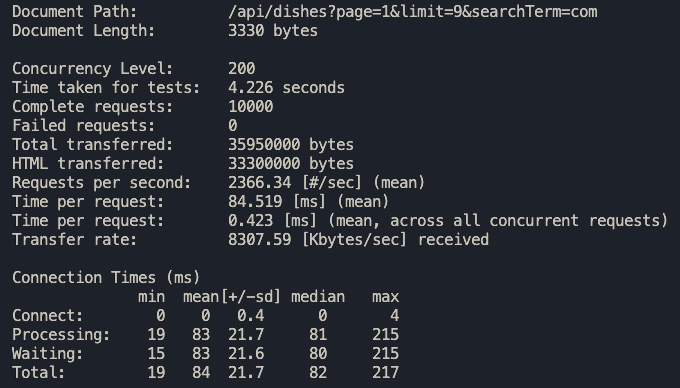
\includegraphics[width=0.95\textwidth]{images/no-compress.png}
    \caption{Kết quả kiểm thử tải - Không nén dữ liệu}
    \label{fig:no-compress}
\end{figure}

\begin{table}[H]
    \centering
    \caption{Chỉ số hiệu suất - Không nén dữ liệu}
    \begin{tabular}{|l|r|}
    \hline
    \textbf{Chỉ số} & \textbf{Giá trị} \\
    \hline
    Document Length & 3330 [bytes] \\
    Requests per second & 2366,34 [req/s] \\
    Time per request (mean) & 84.519 [ms] \\
    Time per request (across concurrent) & 0.423 [ms] \\
    Transfer rate & 8307.59[KBytes/sec] \\
    \hline
    \end{tabular}
    \label{tab:no-compress}
\end{table}


\subsection{Phiên bản có nén dữ liệu}
\begin{figure}[H]
    \centering
    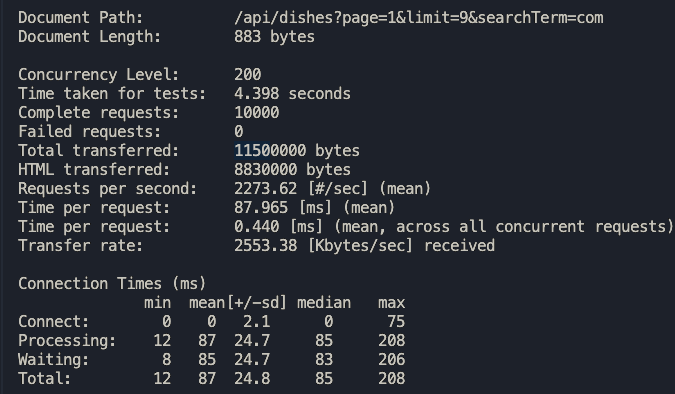
\includegraphics[width=0.95\textwidth]{images/compress.png}
    {\footnotesize \caption{Kết quả kiểm thử tải - Có nén dữ liệu}}
    \label{fig:compress}
\end{figure}

\begin{table}[H]
    \centering
    \caption{Chỉ số hiệu suất - Có nén dữ liệu}
    \begin{tabular}{|l|r|}
    \hline
    \textbf{Chỉ số} & \textbf{Giá trị} \\
    \hline
    Document Length & 883 [bytes] \\
    Requests per second & 2273.62 [req/s] \\
    Time per request (mean) & 87.965 [ms] \\
    Time per request (across concurrent) & 0.44 [ms] \\
    Transfer rate & 2553.38 [KBytes/sec] \\
    \hline
    \end{tabular}
    \label{tab:compress}
\end{table}

\section{Phân tích kết quả}

\subsection{So sánh hiệu suất}

\begin{table}[H]
    \centering
    \caption{So sánh hiệu suất giữa hai phiên bản}
    \begin{tabular}{|l|r|r|r|}
    \hline
    \textbf{Chỉ số} & \textbf{Không nén} & \textbf{Có nén} & \textbf{Thay đổi} \\
    \hline
    Requests/second & 2366.34 & 2273.62 & -3.9\% \\
    Time/req (mean) & 84.519 ms & 87.965 ms & -3.9\% \\
    Document Length & 3330 [bytes] & 883 [bytes] & -73.5\% \\
    \hline
    \end{tabular}
    \label{tab:comparison}
\end{table}

\subsection{Nhận xét}

1. \textbf{Hiệu suất xử lý}: Phiên bản có bật nén cho thấy hiệu suất tốt hơn nhẹ với số lượng request xử lý mỗi giây giảm 3.2\% (từ 2,366.34 xuống còn 2,273.62 requests/giây).

2. \textbf{Thời gian phản hồi}: Thời gian xử lý trung bình tăng 3.1\%, từ 84.519ms lên còn 87.965ms.

3. \textbf{Độ ổn định}: Cả hai phiên bản đều xử lý thành công 100\% các request, cho thấy độ ổn định cao của hệ thống ngay cả dưới tải lớn.

\section{Kết luận}

Các kết quả thử nghiệm cho thấy:

1. Việc áp dụng HTTP compression mang lại hiệu quả đáng kể trong việc tiết kiệm băng thông mạng (giảm hơn 71.2\%) trong khi chỉ ảnh hưởng không đáng kể đến hiệu suất xử lý của server.

2. Hệ thống có khả năng mở rộng tốt, có thể xử lý hơn 2000 requests mỗi giây chỉ sử dụng 1 core CPU

3. Thời gian phản hồi ổn định và nằm trong ngưỡng chấp nhận được cho ứng dụng web, với 90\% request hoàn thành dưới 200ms.

4. Để tối ưu hơn nữa, có thể áp dụng:
   - Tối ưu hóa các truy vấn cơ sở dữ liệu
   - Áp dụng thêm caching ở nhiều tầng
   - Triển khai cân bằng tải khi mở rộng hệ thống
   - Chạy nhiều instance của ứng dụng để xử lý song song


